\documentclass[lettersize,journal]{IEEEtran}
\usepackage{amsmath,amsfonts}
\usepackage{algorithmic}
\usepackage{algorithm}
\usepackage{array}
\usepackage[caption=false,font=normalsize,labelfont=sf,textfont=sf]{subfig}
\usepackage[shortlabels]{enumitem}
\usepackage{textcomp}
\usepackage{stfloats}
\usepackage{url}
\usepackage{verbatim}
\usepackage{graphicx}
\usepackage{cite}
\usepackage{bm}
\hyphenation{op-tical net-works semi-conduc-tor IEEE-Xplore}


\begin{document}

\title{ECE 552: Project Status Report\\ Micro-architectural Support for Packed Sparse Matrix Multiplication on Hybrid Systolic Arrays}

\author{David Raibaut}

\maketitle
\begin{abstract}
    This project pulls inspiration from two novel architectural methods for increasing NPU efficiency: Hybrid Systolic Arrays (HSA) \cite{HSA-paper} and Sparse-TPU \cite{sparse-tpu}.
    HSA provides a way of reducing chip area by combining matrix and vector multiplies into a single systolic array. Sparse-TPU provides hardware support for sparse-packed matrices
    thus increasing performance and reducing area. I will develop unit tests and benchmarks for the components to ensure functional correctness, compare HSA, sparse-tpu and their novel combination with more traditional
    methods and analyze the performance and energy efficiency impact.
\end{abstract}

% \begin{IEEEkeywords}
% Article submission, IEEE, IEEEtran, journal, \LaTeX, paper, template, typesetting.
% \end{IEEEkeywords}

\section{Introduction and Problem Statement}
User demand for Large Language Model (LLM) inference has grown rapidly throughout the past years \cite{LLM-demand-growth}.
On-edge inference has emerged as a powerful alternative to cloud-based solutions,
thanks to its lower cost, decreased latency and heightened security with comparable
performance for daily tasks. However, the limited memory capacity, energy constraints
and sequential query model pose significant challenges for successfully deploying
LLMs on edge, where user-facing applications require minimal latency (dictated by the decode stage \cite{HSA-paper})
and a reduced energy footprint (dictated by external memory accesses (EMA)) \cite{HSA-paper}.

A proposed solution is the use of sparse-matrix LLMs \cite{sparse-tpu}, such as SparseLLM \cite{sparse-llm},
SparseGPT \cite{sparse-gpt} and KMZ \cite{KMZ}. These models compress larger trained models to reduce
their number of parameters and hence reduce the memory requirements
for the model and the number of operations to produce their
computation by making their composing matrices sparser.

Other proposals to enhance edge inference efficiency include the use of Hybrid Systolic Arrays (HSA) \cite{HSA-paper}.
These units function as an intermediate point between Matrix Processing Units (MPU, used during pre-fill stage)
and Vector Processing Units (VPU, used during decode stage), thus eliminating the need for both.
This has been shown to effectively reduce the area and thus energy consumption and maintain
comparable latency.

In this project I plan to explore a novel HSA, by including hardware support for packed sparse matrices,
essentially exploring the performance-efficiency tradeoff exposited by a combination of two previous methods.
I will also implement sparse-matrix support on clock-gated MPUs and VPUs to show the advantage provided by
the HSA architecture, and conversely non-sparse matrix supported MPUs, VPUs and HSAs to show the advantage provided by the HSA structure independently.

\section{Related Work}
There have been multiple proposals for on-edge LLM inference without the use of dedicated hardware accelerators,
focusing mostly on CPU optimisation \cite{cpu-outperform-on-device-llm-inference}, \cite{enhancing-llm-inference-on-arm-cpu}, \cite{efficient-llm-inference-on-cpu},
efficient model compression and quantization \cite{advances-low-bit-quant-llm-edge}, \cite{how-to-run-large-ai-model-edge-device} and
even custom frameworks for edge-specific model design \cite{llama.cpp}, \cite{media-pipe}.

Even then, due to the tight energy and performance efficiency constraints on edge devices, particularly mobile devices such as phones or wearables,
most of these techniques incur large tradeoffs, such as requiring models to be very small \cite{cpu-outperform-on-device-llm-inference} ($\sim$1B parameters), 
or finding significant performance degradation at sub-4-bit quantization \cite{advances-low-bit-quant-llm-edge}.

Thus, given the rise in user-demand \cite{LLM-demand-growth} for low-latency high-performing LLMs, the most likely path forward seems to be dedicated
hardware accelerators \cite{google-seminal-paper} optimised for this specific workload.

In this project I will mostly refer to the HSA \cite{HSA-paper} and Sparse-TPU \cite{sparse-tpu} as they are the two most relevant sources due
to their closeness with the proposed implementation. Other notable areas of research include heterogeneous systems \cite{heterogeneous}, \cite{NPU-PIM}, as a way of attempting to reduce
the memory bandwidth bottleneck at the cost of architectural flexibility, compressed KV-cache implementations \cite{kv-cache-compressed} at the cost of added latency
and KV cache reuse optimisations \cite{kv-cache-reuse} at the cost of decreased accuracy.

\section{Research Questions}
\begin{itemize}
    \item How can existing HSA hardware be adapted to support packed sparse matrix multiplication?
    \item How much performance and energy gains does packed sparse matrices provide in practice?
    \item How much performance and energy gains does HSAs provide in practice?
    \item How much performance and energy gains does the novel packed sparse matrix HSAs provide in practice?
\end{itemize}

\section{Proposed Solutions}
% Modifications
%% - VPU: adding pipelining, demux broadcast channels
%% - Sparse: double-pumped columns
%% - HSA: Choose one or other mode (mux)
%% - SMPU: double pump columns?
%% - SHSA: combine - for MMM how to double pump columns?
The proposed solution is that of a HSA structure with added hardware support for sparse-packed matrices.
The use of the HSA structure allows for a lower chip area (since separate MPUs and VPUs are not required
for the pre-fill and decode stages respectively) thus leading to lower leakage power and overall
energy use. Hardware-support for sparse-packed matrices increase performance by significantly reducing the number
of operations required to be computed (i.e. the number of MAC units), at the cost of some accuracy (due to the packing), and thus
reducing overall SA latency. Moreover, by clock-gating the individual MAC units, the dynamic power of
the whole chip can be reduced thus decreasing energy use too.

In this project I set out to explore whether this novel idea of a HSA with support for sparse-packed matrices (referred to throughout as SHSA)
truly leads to the performance and energy improvements over single HSA or single sparse-packing, how much each
of these individual improvements contributes and what the accuracy tradeoff is.

\subsection{Vector, Matrix and Hybrid Dataflows in Detail}
The VPU performs Matrix-Vector Multiplication (MVM) during the decode stage,
and the MPU performs Matrix-Matrix Multiplication (MMM) during the pre-fill stage.
There are many dataflows possible for these different operations, all functionally equivalent,
but with different tradeoffs. The two most salient type of dataflows are:

\begin{itemize}
    \item Output-stationary (OS): each MAC is responsible of holding the matrix entry at its position,
        where the weight and activation data `flow' over the architecture
    \item Weight-stationary (WS aka HSA-style): each MAC is pre-loaded with its weight value and the activation and partial
        sums flow over the MAC array, with the final answer being received in waves at the end of the MAC array.
\end{itemize}
Because a HSA unit should be able to operate both MVM and MMM operations, the microarchitecture
for the MPU and VPU units should be similar enough that they could be hybridised.

I have decided to implement all my units in WS mode for the following reasons:
\begin{enumerate}
    \item Minimise EMA during decode stage. In output stationary, each cycle weights are streamed leading to longer latencies
        or larger bandwidth, as during the decode stage I use $\mathcal{O}(1)$ activations but $\mathcal{O}(N)$ weights. In a WS
        model I can reuse the loaded weights across operations or pipeline their loading and save bandwidth.
    \item OS would mean $\mathcal{O}(N^2)$ MACs. Although this would be fine
        during pre-fill, there would be significant under-utilisation of resources during the decode stage, where at most $\mathcal{O}(N)$ values are being calculated.
        \emph{Note:} This is also true to some extent for the WS model, but MAC units can be gated trivially and moreover I have found a way to pipeline
        the vector multiplications in a weight-stationary model to incur negligible under-utilisation (see figure \ref{wavefronts}).
    \item OS would require significant differences in the dataflow and gating style in MVM and MMM modes for the HSA unit
        leading to more complex control circuitry reducing the area and energy advantages that the hybrid approach provides.
\end{enumerate}
Thus I have opted for a WS dataflow model. My proposed method has the systolic `wavefront' move
diagonally for MMM units and horizontally for MVM units (note: there is also a way to eliminate weight-loading
wavefronts if we can reuse weights across operations). This is what has allowed me to pipeline the weight-loading,
since at any given instance only units on the wavefront (i.e. a column for MVM or a diagonal for MMM) are being operated.
See figure \ref{wavefronts} for a graphical representation.

\begin{figure*}[!t]
    \centering
    \includegraphics[width=0.75\textwidth]{MMM_pipes.png}
    \caption{The pipelining model I came up with to mitigate the under-utilisation. Shown is the MMM mode, which is the most
    complex, the MVM is identical except wavefronts are columns as opposed to diagonals. The arrows show the flow of partial sums
    (can be either horizontal or vertical, but I typically take it to be horizontal) and partial sums (taken here to be left to right).
    The `master' circuit driving this MPU/VPU is responsible of keeping track and reading the outputs for each of the different
cycles when they are ready}
    \label{wavefronts}
\end{figure*}

\subsection{Packed vs non-packed dataflows}
The original STPU paper \cite{sparse-tpu} proposes a more flexible approach to handling sparse-matrix packing than traditional fixed-packed 2:1 methods.
However, in doing this, significant complexity is introduced for the sake of maintaining the flexibility of a variable sparsity factor which does not
map well onto the hybrid architecture.

Moreover, the paper introduces sparse-matrix packing for the decode stage, since MMM operations
introduce significant structural hazards in the systolic data flow, which is why I have adapted my roadmap to eliminate the sparse-MPU unit,
as implementing such a unit is well beyond the scope of this project.

Due to the increased complexity of the original STPU paper, I have proceeded to create my own more simplified approach for adapting VPUs and HSA (in MVM mode).
This novel method, although incurring a slight loss in accuracy, allows for either a $\sim$2x gain in performance or a $\sim$2x gain in energy saving, with only
a slight increase in die area.

The crux of the packed (sparse) vs non-packed microarchitectures is as follows.
Suppose we are working with a sparse model (i.e. weights have been pruned during training)
with the following weights matrix:
\begin{equation*}
    W = \begin{bmatrix}
        5 & 0 & 1 & 7 \\
        0 & 4 & 0 & 1 \\
        0 & 2 & 5 & 0 \\
        4 & 0 & 0 & 0
    \end{bmatrix}
\end{equation*}
On a WS model, any 0-weight entry would map to an essentially
idle MAC unit.
To reduce the sparsity, we pack the matrix through column merging: Each
element's row is kept invariant and elements must be tagged
with the column they came from. This allows for correction of
the severe underutilisation of MAC units. However, I noticed
two key things:
\begin{itemize}
    \item Reducing EMA is our priority. Since most models are low-bit
        quantized ($Q < 8$), adding 
        tags increases EMA if $Q < \log_2 N$.
        Since weight matrices are typically large ($N \sim 2^{10}-2^{14}$ for small models),
        including tags guarantees added EMA and latency.
    \item Since each MAC now may need to keep track of values from multiple different
        columns and make sure they match with the activation value,
        MAC complexity increases.
\end{itemize}
So, my simplification is to merge only adjacent columns, and discard the lower-valued weight arbitrarily.
Since we only merge adjacent columns, columns now need to be tagged solely with the parity of their
column index (one bit) and the need for additional memory elements in each MAC is eliminated. For example,
the matrix above would become:
\begin{equation*}
    W = \begin{bmatrix}
        5,0 & 7,1 \\
        4,1 & 1,1 \\
        2,1 & 5,0 \\
        4,0 & 0,0
    \end{bmatrix}
\end{equation*} 
% There is some added complexity in this case: where before each cycle a single activation value
% was broadcast to each column in our MAC array, now two different activation values must be broadcast,
% since for example, for $A = [4\;8\; 12\; 16]$, during the first cycle both $4$ and $8$ must be broadcast
% to the first column since the units holding $5,0$ and $4,0$ need the activation value $4$ whereas
% $4,1$ and $2,1$ would need $8$. However, the key to notice here is that no new buses must be added
% to broadcast these values, since we have essentially collapsed our horizontal dimension in two (so the
% doubling of busses cancels out).

The only added tradeoffs we incur with my simplification is the following:
\begin{itemize}
    \item Slight reduction in accuracy from sparse packing: for example, in above matrix, row 1's column 3's value had to be dropped.
    \item 1 additional EMA per cycle, as each column now needs 2 activation values, which can be achieved with an extra read port to the activation memory, which is negligible in comparison
        with the $\mathcal{O}(N)$ accesses for weights.
    \item 1 additional input port and mux in each of the MACs: the additional input port is for the second activatino value, and the mux
        will use the column parity tag as a select bit so that the appropriate activation value is used for the multiplication. This is far less than the
        added MAC complexity from the STPU paper.
\end{itemize}
\section{Evaluation - Current Status}
\subsection{Methodology}
The hardware units will be implemented in both a C++ software simulator (custom-built from scratch, cycle accurate)
as well as SystemVerilog \cite{sys-verilog} modules,
with Xilinx Vivado to synthesize them.
They will be tested on the AMD Artix A7 FPGA with 63400 LUTs, 126800 FFs, and 4860Kb of SRAM. 
Given the memory and logic slice constraints on the Artix A7, I estimate I will be able to fit a 32 by 32 SA unit, along with the accompanying driving logic, however this is subject to change.
Assuming this, the weight and activation SRAMs will be 64kB and 4kB each in total.
\begin{table}[]
    \centering
    \caption{Project status}
    \begin{tabular}{|l|l|l|}
    \hline
    Unit   & C++?   & Verilog? \\ \hline
    MAC-WS & FV     & FV       \\ \hline
    MAC-OS & FV     & NS       \\ \hline
    VPU-OS & FV     & NS       \\ \hline
    MPU-OS & FV     & NS       \\ \hline
    VPU-WS & FV     & FV       \\ \hline
    MPU-WS & FV     & NS       \\ \hline
    HSA    & FV     & NS       \\ \hline
    SVPU   & S-50\% & NS       \\ \hline
    SHSA   & NS     & NS       \\ \hline
    NPU\footnotemark
        & NS     & NS       \\ \hline
    \end{tabular}
       
    \label{project-status-table} 
\end{table}
\footnotetext{Due to the large ambition and scope of this project,
    implementing the NPU unit has been moved to a secondary
    objective, as this is not critical in showing the performance
    difference between different VPU/MPU/HSA units, but rather
    a `bells-and-whistles' unit required to run an actual LLM model
    such as RetNet on the units. They can instead be benchmarked
    using matrices directly extracted from the weight/activation values
    of such models.
}


Table \ref{project-status-table} shows the status of the units being implemented.
An `FV' indicates units that have been implemented and functionally
validated (to a large extent, but not exhaustively - this will come at a later
milestone), a `NS' indicates
a unit that has not yet been started, and a `S-P\%' indicates
a unit that has been started and is P\% percent of the way there.

Figure \ref{2x2-hvpu} shows an 2x2 MAC circuit  of the HVPU
implementation in verilog as generated by Vivado, and figure
\ref{2x2-hvpu-trace} shows such a unit correctly
performing the operation:
\begin{equation*}
    \begin{bmatrix}
        2 & 3\\
        4 & 5
    \end{bmatrix}
    \begin{bmatrix}
        2\\
        1
    \end{bmatrix} = \begin{bmatrix}
        7\\
        13
    \end{bmatrix}
\end{equation*} 
As you can see, this unit correctly implements the pipelined weight loading that was
previously mentioned. \emph{Note:} The unit size (i.e. rows and columns
of MAC units) and bus bit width was parametrised in Verilog.
\begin{figure*}[!t]
    \centering
    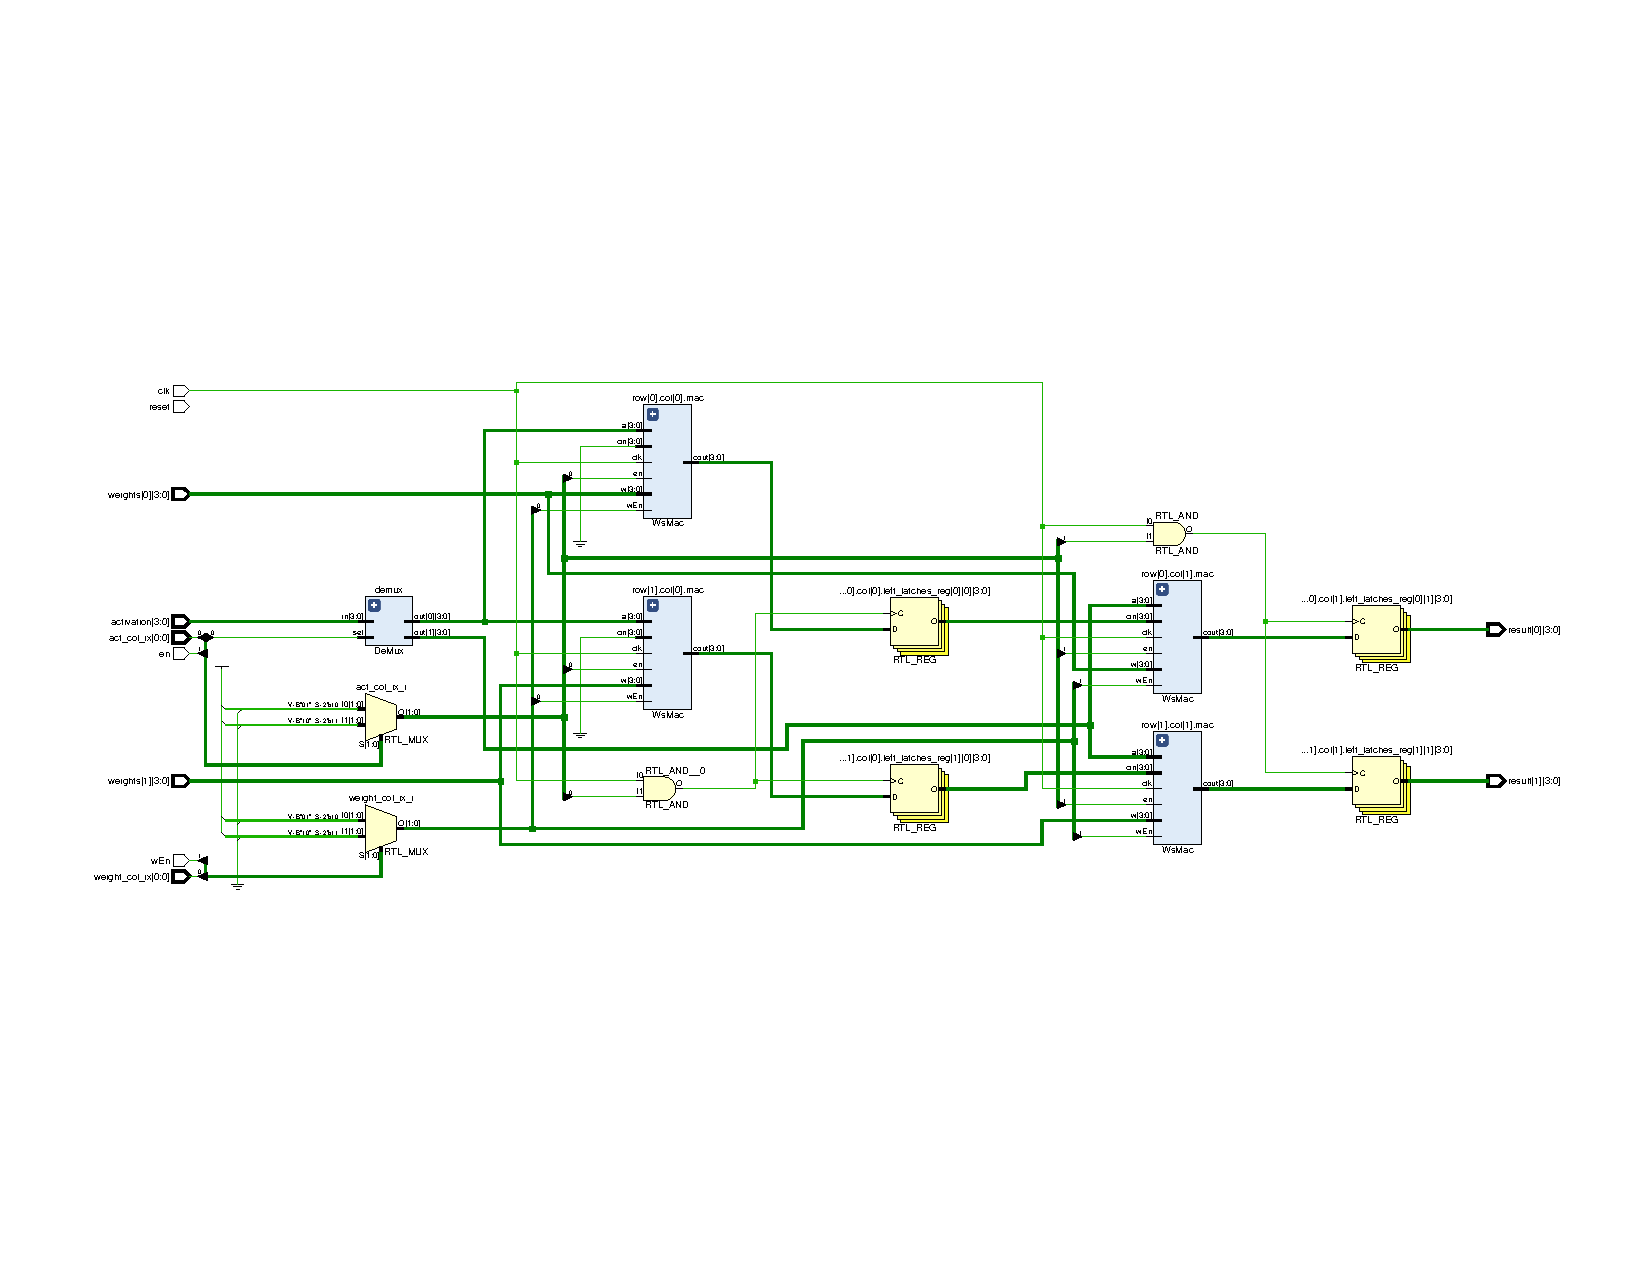
\includegraphics[width=0.8\textwidth]{HVPU_2x2.jpg}
    \caption{The 2x2 VPU-WS unit running on 4-bit quantisation}
    \label{2x2-hvpu}

\end{figure*}
\begin{figure}[!t]
    \centering
    \includegraphics[width=2.5in]{2x2-hvpu-trace.png}
    \caption{2x2 VPU-WS trace showing functional validity}
    \label{2x2-hvpu-trace}
\end{figure}

You can access the GitHub repo for this project
to see all my work so far ($\sim$ 1000 lines of C++,
and $\sim$ 200 lines of verilog) at this link:
\url{https://github.com/DR-Reg/ECE-552-project}
 
%% Progress (*=start,^=not start,B=bells&whistles):
% CPP_IMPL: HVPU, HMPU, VPU, MPU, HSA, SVPU*, SMPU^, SHSA^, NPU^B
% VERILOG: HVPU, ---  
\subsection{Functional Validation}
\begin{enumerate}[(a)]
    \item \emph{Unit testing}: Test benches in SystemVerilog will be provided for each of the aforementioned units. Currently the single VPU-WS unit (called VpuHsa.v) has an accompanying test bench (VpuHsa\_tb.v), with the rest of units pending.
    \item \emph{Software implementation}: The C++ implementation itself has been made cycle accurate and has been functionally
        validated and traced by hand for all units that have been implemented so far ($\sim$90\% of units). Most of the important
        files for this can be found in cpp\_impl/include
\end{enumerate}
\subsection{Physical Characteristics}
Vivado software provides tools for finding power: both compiler estimates and XADC System Monitor readings will be provided for power.

Vivado also provides tools for assessing the maximal frequency, namely the timing report after synthesis,
which includes the `Worst Negative Slack' (WNS) metric. In the case of a negative WNS,
an analysis of the critical paths and iterative redesign/testing will be performed,
until all designs meet the timing requirements. Ideally, all structures should operate at the same frequency, since
supporting NPU package (either hardware implemented or software emulated) will be identical as control variables. However, in the case that they are not clocked equally,
start-to-end latency and total energy expenditure will be used as the performance metrics.

Vivado synthesis also provides data for logic cell and BRAM utilisation which will be used as an estimate for chip area.

\subsection{Performance Impact}
Performance impact will be compared across multiple metrics:
\begin{enumerate}
    \item Accuracy (for sparse-packing, \% diff vs non-packed)
    \item Raw performance (TOPS)
    \item Energy efficiency (pJ/Token)
    \item Power efficiency (TOPS/W)
    \item Area (mm2) - directly from Vivado
\end{enumerate}
Raw performance will be approximated by estimating the operations per clock cycle (or simply
end-to-end latency in seconds in the case where different frequencies have to be used),
and energy efficiency will be calculated from the power efficiency (which can be estimated
using Xilinx's XPower tool). Accuracy can be found by computing the percent-difference
per-element between packed and non-packed results.
\section{Revised Milestones}
A slight modification is done to the milestones, since the NPU supporting package has become a secondary
priority:
\begin{enumerate}
    \item \textbf{Milestone 1: C++ Software Implementation (90\% done):} I expect to finish this by the end of this week 
    \item \textbf{Milestone 2: Unit Implementation in Verilog (15\% done):} I expect to finish this by the middle of next week 
    \item \textbf{Milestone 3: Functional Validation and Performance Testing (40\% done):} I have been validating my units as I made them,
        but formal validation will be performed once all units are finished and performance metrics extracted.
    \item \textbf{Milestone 4: Final Evaluation and Reporting (Not Started):} Analyze performance and write report, once milestone 3 is finished.
    \item \textbf{Bells and Whistles: NPU Package (Not Started)} If possible, get these units to work so I can showcase my hardware accelerator running
        a real workload start to finish.
\end{enumerate}
Although it may seem I am slightly behind with respect to my original planning, I am in fact ahead,
since my decision to make the C++ software implementation cycle accurate means that the software
is almost a 1:1 representation of the hardware, so making the Verilog modules takes significantly less
time (1-2h per unit). Making the C++ implementation has allowed me to refocus the project to a
novel idea for architectural support of packed matrices and is more realisable in the given time frame.
\section{Division of Labour}
All work has been and will continue to be done by me (David Raibaut).
\section{References}
% You can use a bibliography generated by BibTeX as a .bbl file.
%  BibTeX documentation can be easily obtained at:
%  http://mirror.ctan.org/biblio/bibtex/contrib/doc/
%  The IEEEtran BibTeX style support page is:
%  http://www.michaelshell.org/tex/ieeetran/bibtex/
 
 % argument is your BibTeX string definitions and bibliography database(s)
%\bibliography{IEEEabrv,../bib/paper}
%
% \section{Simple References}
% You can manually copy in the resultant .bbl file and set second argument of $\backslash${\tt{begin}} to the number of references
%  (used to reserve space for the reference number labels box).
\bibliographystyle{IEEEtran}
\bibliography{IEEEabrv,refs}
\vfill

\end{document}


